\begin{frame}
	\frametitle{A elasticidade como medida}
	\begin{itemize}
		\item A elasticidade \'e uma medida da varia\c c\~ao percentual de uma vari\'avel como resposta \`a varia\c c\~ao percentual da outra.
		\item Em \underline{termos discretos}, e considerando uma situa\c c\~ao inicial representada pelo ponto $(x_1,y_1)$ e uma situa\c c\~ao final representada pelo ponto $(x_2,y_2)$, a elasticidade de $Y$ em rela\c c\~ao a $X$ ser\'a calculada como \[\frac{\Delta\% \text{ em } Y}{\Delta\% \text{ em } X}=\frac{\frac{\Delta Y}{y_1}\times 100}{\frac{\Delta X}{x_1}\times 100}=\frac{\Delta Y}{\Delta X}\times\frac{x_1}{y_1}\]
	\end{itemize} 

	Onde $\Delta Z = z_2-z_1$.

\end{frame}

\begin{frame}
	\frametitle{A elasticidade como medida}
	\begin{itemize}
		\item Em \underline{termos cont\'inuos}, e conhecendo $Y=f(X)$, a elasticidade de $Y$ em rela\c c\~ao a $X$ ser\'a calculada como \(\frac{d Y}{d X} \frac{X}{Y}\)
		\item Vamos estudar as seguintes elasticidades:
	\end{itemize}
	\vspace{0.2cm}
	\begin{columns}
		\begin{column}{0.50\textwidth}
			{\color{blue} Elasticidades da procura}
			\begin{itemize}
				\item[$\varepsilon_{D}$] Pre\c co - direta da procura
				\item[$\varepsilon_{x,y}$] Pre\c co cruzada da procura
				\item[$\eta$] Rendimento da procura
			\end{itemize}
		\end{column}
		\begin{column}{0.47\textwidth}
			{\color{blue} Elasticidades da oferta}
			\begin{itemize}
				\item[$\varepsilon_{S}$] Pre\c co da Oferta
			\end{itemize}
			\vspace{1cm}
		\end{column}
	\end{columns}
\end{frame}

\begin{frame}
	\frametitle{A elasticidade como medida}
	As elasticidades da procura medem a varia\c c\~ao percentual da quantidade procurada quando h\'a uma varia\c c\~ao percentual de outra vari\'avel que a influencia. S\~ao o reflexo da sensibilidade do consumidor face a essa vari\'avel.
\end{frame}

\begin{frame}
	\frametitle{A elasticidade como medida}

		Elasticidade Pre\c co-Directa: \'e a varia\c c\~ao percentual da quantidade procurada quando h\'a uma varia\c c\~ao percentual do pre\c co do mesmo bem, ou seja: \[\varepsilon_D=\frac{\Delta\%Q_D}{\Delta\%P}=\frac{\frac{\Delta Q_D}{Q_D}}{\frac{\Delta P}{P}}={\color{blue}\frac{\Delta Q_D}{\Delta P}\frac{P}{Q_d}=\frac{dQ_D}{dP}\frac{P}{Q_d}}\]

		Mas $Q_D=a-bP$, assim $\frac{dQ_D}{dP}=-b$, assim em geral, $\varepsilon_D<0$

\end{frame}

\begin{frame}
	\frametitle{A elasticidade como medida}
	Classifica\c c\~ao da procura quanto \`a $\varepsilon_D$:
	\begin{itemize}
		\setlength\itemsep{0.5cm}
		\item $|\varepsilon_D|>1$ $\Rightarrow$ a procura \'e el\'astica
		\item $|\varepsilon_D|=1$ $\Rightarrow$ a procura tem elasticidade unit\'aria
		\item $|\varepsilon_D|<1$ $\Rightarrow$ a procura \'e inel\'astica ou r\'igida
	\end{itemize}

\end{frame}

\begin{frame}
	\frametitle{Elasticiade Pre\c co da Procura}

	$Q_D=100-5P$ para a forma linear $Q_D=a-b\times P$

	\begin{center}
		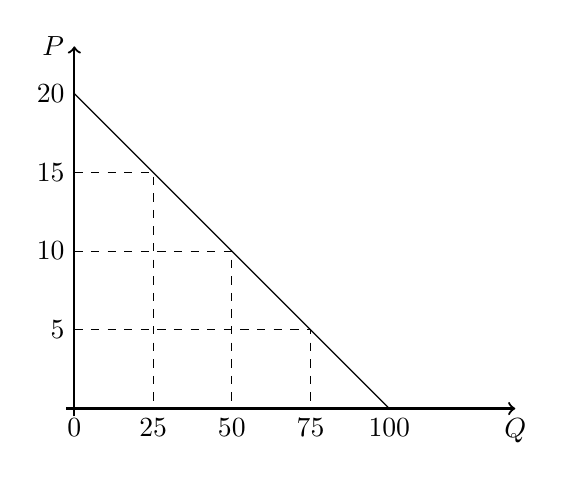
\begin{tikzpicture}[
			scale = 1,
			every node/.style = {scale = 1},
			declare function ={
				d(\x) = 4-\x;
			}
			]

			\draw[->,thick] (-0.1,0) -- (5.6,0)node[below]{$Q$};
			\draw[->,thick] (0,-0.1) -- (0,4.6)node[left]{$P$};

			\draw[domain=0:4,variable=\x] plot (\x,{d(\x)})node[below]{$100$};

			\foreach \n/\m in {5/75,10/50,15/25,20/0}{
				\draw[dashed](0,{\n/5})node[left]{$\n$} -- ({d(\n/5)},{\n/5}) -- ({d(\n/5)},0)node[below]{$\m$};
			}

		\end{tikzpicture}
		\par
		Qual a elasticidade pre\c co-directa na procura quando $P=15$? e $P=10$? e $P=5$?
	\end{center}

\end{frame}

\begin{frame}
	\frametitle{Elasticidade Pre\c co-Directa}
	\[\varepsilon_D=\frac{\Delta\% Q_D}{\Delta\% P}=\frac{\frac{\Delta Q_D}{q}}{\frac{\Delta P}{p}}=\frac{\Delta Q_D}{\Delta P}\frac{p}{q}\]
	No nosso caso:\[Q_D=100-5P\quad\Rightarrow\quad\Delta Q_D=-5\Delta P\] Logo \[\frac{\Delta Q_D}{\Delta P}=-5\]
\end{frame}

\begin{frame}
	\frametitle{Elasticidade Pre\c co-Directa}
	Quando $P=15$, $Q=25$, Logo:\[\varepsilon_D=\frac{\Delta \% Q_D}{\Delta \% P}=\frac{\frac{\Delta Q_D}{q}}{\frac{\Delta P}{p}}=\frac{\Delta Q_D}{\Delta P}\frac{p}{q}=-5\times\frac{15}{25}=-3\]
	Quando $P=15$, se o pre\c co aumentar 1\%, a quantidade procurada reduz-se 3\%.\par
	Como $|\varepsilon|>1$, diz-se que, neste ponto, a procura \'e \textbf{el\'astica}.
\end{frame}

\begin{frame}
	\frametitle{Elasticidade Pre\c co-Directa}
	Quando $P=5$, $Q=75$, Logo:\[\varepsilon_D=\frac{\Delta \% Q_D}{\Delta \% P}=\frac{\frac{\Delta Q_D}{q}}{\frac{\Delta P}{p}}=\frac{\Delta Q_D}{\Delta P}\frac{p}{q}=-5\times\frac{5}{75}=-0.33\]
	Quando $P=5$, se o pre\c co aumentar 1\%, a quantidade procurada reduz-se 0.33\%.\par
	Como $|\varepsilon|<1$, diz-se que, neste ponto, a procura \'e \textbf{inel\'astica}.
\end{frame}

\begin{frame}
	\frametitle{Elasticidade Pre\c co-Directa}
	Quando $P=10$, $Q=50$, Logo:\[\varepsilon_D=\frac{\Delta \% Q_D}{\Delta \% P}=\frac{\frac{\Delta Q_D}{q}}{\frac{\Delta P}{p}}=\frac{\Delta Q_D}{\Delta P}\frac{p}{q}=-5\times\frac{10}{50}=-1\]
	Quando $P=5$, se o pre\c co aumentar 1\%, a quantidade procurada reduz-se 1\%.\par
	Como $|\varepsilon|=1$, diz-se que, neste ponto, a procura tem elasticidade \textbf{unit\'aria}.
\end{frame}

\begin{frame}
	\frametitle{Elasticiade Pre\c co da Procura}

	$Q_D=100-5P$ para a forma linear $Q_D=a-b\times P$

	\begin{center}
		\begin{tikzpicture}[
			scale = 0.8,
			every node/.style = {scale = 0.7},
			declare function ={
				d(\x) = 4-\x;
			}
			]

			\draw[->,thick] (-0.1,0) -- (5.6,0)node[below]{$Q$};
			\draw[->,thick] (0,-0.1) -- (0,4.6)node[left]{$P$};

			\draw[domain=0:4,variable=\x] plot (\x,{d(\x)})node[below]{$100$};

			\onslide<1-4>{
				\foreach \n/\m in {5/75,10/50,15/25,20/0}{
					\draw[dashed](0,{\n/5})node[left]{$\n$} -- ({d(\n/5)},{\n/5}) -- ({d(\n/5)},0)node[below]{$\m$};
				}
			}

			\onslide<2->{
				\draw(2,2)node[circle,fill=red,inner sep=2,label=above right:{\(|\varepsilon_D|=1\)}]{};
			}

			\onslide<3-4>{
				\draw[pen colour={red},ultra thick,decorate,decoration={calligraphic brace},yshift=0.1cm,xshift=0.1cm] (2,2) -- (4,0) node[midway,xshift=1cm,yshift=0.1cm]{$|\varepsilon_D|<1$};
			}

			\onslide<4-4>{
				\draw[pen colour={red},ultra thick,decorate,decoration={calligraphic brace},yshift=0.1cm,xshift=0.1cm] (0,4) -- (2,2) node[midway,xshift=0.75cm,yshift=0.25cm]{$|\varepsilon_D|>1$};
			}

			\onslide<5-6>{
				\draw(0,4)node[circle,fill=green,inner sep=2]{};
			}

			\onslide<6>{
				\draw(3.5,4)node[]{$|\varepsilon_D|=\left|\frac{\Delta Q_D p}{\Delta P q}\right|=\lim_{x\rightarrow0}5\times\frac{20}{x}=+\infty$};
			}

			\onslide<7-8>{
				\draw(4,0)node[circle,fill=blue,inner sep=2]{};
				\draw(0,4)node[circle,fill=green,inner sep = 2,label=above right:{\(|\varepsilon_D|=+\infty\)}]{};
			}

			\onslide<8>{
				\draw(5,3)node[]{$|\varepsilon_D|=\left|\frac{\Delta Q_D p}{\Delta P q}\right|=\lim_{x\rightarrow0}5\times\frac{0}{100}=0$};
			}

			\onslide<9>{
				\draw(4,0)node[circle,fill=blue,inner sep=2,label=above right:{\(|\varepsilon_D|=0\)}]{};
				\draw(0,4)node[circle,fill=green,inner sep = 2,label=above right:{\(|\varepsilon_D|=+\infty\)}]{};
			}

		\end{tikzpicture}
	\end{center}
		\par
		Ao longo de uma procura linear, a elasticidade vai-se alterando. \onslide<5-8>{\color{green!80!black} Qual \'e a elasticidade no ponto verde?}\onslide<7-8>{\color{blue} e no ponto azul?}
\end{frame}

\begin{frame}
	\frametitle{Elasticidade Pre\c co-Directa}
	Quanto maior $|\varepsilon_D|$ mais o consumidor \'e sens\'ivel \`as varia\c c\~oes de pre\c co:
	\begin{itemize}
		\item Se \'e muito sens\'ivel, ent\~ao a procura \'e el\'astica e a quantidade reage de forma mais do que proporcional em rela\c c\~ao \`a varia\c c\~ao de pre\c co.
		\item Se \'e pouco sens\'ivel, ent\~ao a procura \'e inel\'astica e a quantidade reage de forma menos do que proporcional em rela\c c\~ao \`a varia\c c\~ao de pre\c co.
	\end{itemize}
\end{frame}

\begin{frame}
	\frametitle{Factores que influenciam a Elasticidade Pre\c co-Directa da Procura}
	\begin{itemize}
		\setlength{\itemsep}{0.3cm}
		\item Peso que a despesa de um bem tem no or\c camento para consumo
		\item Exist\^encia de mais bens substitutos
		\item Per\'iodo de tempo
	\end{itemize}
\end{frame}

\begin{frame}
	\frametitle{Elasticidade Pre\c co-Directa da Procura: Peso da despesa no or\c camento}
	Quanto maior o peso que a despesa de um bem tem no or\c camento para consumo, mais sens\'ivel ser\'a o consumidor \`as varia\c c\~oes de pre\c co, logo maior ser\'a a elasticidade.\pause
	\par
	\vspace{0.5cm}
	\'E natural, portanto,que as procuras lineares tenham uma zona el\'astica na parte superior, ou seja, quando os pre\c cos unit\'arios ultrapassam certo limiar...
\end{frame}
\begin{frame}
	\frametitle{Elasticidade Pre\c co-Directa da Procura: Exist\^encia de bens substitutos}
	A exist\^encia de mais bens substitutos, aumenta a elasticidade da procura de um bem:
	\begin{itemize}
		\item A elasticidade da procura de leite \'e inferior \`a elasticidade da procura de chantilly.
		\item \textbf{Consequ\^encia 1:} quanto mais espec\'ifica for a defini\c c\~ao de um bem, maior a elasticidade da procura.
		\item[*] A elasticidade da procura de leite \'e menor do que a elasticidade da procura de leite marca $X$.
		\item \textbf{Consequ\^encia 2:} bens essenciais com poucos substitutos t\^em procuras mais r\'igidas:
		\item[*] A elasticidade da procura de p\~ao \'e menor do que a elasticidade da procura de bolos.
	\end{itemize}
	
\end{frame}

\begin{frame}
	\frametitle{Elasticidade Pre\c co-Directa da Procura: Per\'iodo de tempo}
	Per\'iodo de tempo: a elasticidade tende a aumentar com o tempo decorrido, devido \`a possibilidade dos consumidores se conseguirem adaptar \`as varia\c c\~oes de pre\c co:
	\begin{itemize}
		\item A procura de curto-prazo de transporte em autocarro ter\'a uma elasticidade menor do que a procura de longo-prazo.
	\end{itemize}
\end{frame}

\begin{frame}
	\frametitle{Casos extremos}
	\begin{columns}
		\begin{column}{0.47\textwidth}
			\begin{center}
				\begin{tikzpicture}[
					scale = 0.7,
					every node/.style = {scale = 0.7},
					declare function ={
						d(\x) = 4-\x;
					}
					]

					\draw[->,thick] (-0.1,0) -- (5.6,0)node[below]{$Q$};
					\draw[->,thick] (0,-0.1) -- (0,4.6)node[left]{$P$};

					\draw(2,0)node[below]{$Q_0$} -- (2,4)node[midway,xshift=0.25cm]{$D$};

					\onslide<4->{
						\draw(3,1)node[right]{$|\varepsilon_D|=0$};
					}

				\end{tikzpicture}
			\end{center}
			{\scriptsize{
			\onslide<2->{\textbf{A quantidade procurada \'e independente do pre\c co} (para um intervalo de pre\c cos relevante)}\par
			\onslide<3->{(Ex: qualquer bem indispens\'avel \`a sobreviv\^encia e sem substitutos.. e.g.: medica\c c\~ao para doentes cr\'onicos)}
			}
			}
		\end{column}
		\begin{column}{0.47\textwidth}
			\begin{center}
				\begin{tikzpicture}[
					scale = 0.7,
					every node/.style = {scale = 0.7},
					declare function ={
						d(\x) = 4-\x;
					}
					]

					\draw[->,thick] (-0.1,0) -- (5.6,0)node[below]{$Q$};
					\draw[->,thick] (0,-0.1) -- (0,4.6)node[left]{$P$};

					\draw(0,2)node[left]{$P_0$} -- (4,2)node[midway,yshift=0.25cm]{$D$};

					\onslide<6->{
						\draw(3,1)node[right]{$|\varepsilon_D|=\infty$};
					}

				\end{tikzpicture}
			\end{center}
			
			\onslide<5->{
				\scriptsize{
				Os consumidores s\'o compram o bem ao pre\c co $P_0$. Se o pre\c co for maior, n\~ao compram e v\~ao procurar uma alternativa id\^entica mais barata.\par
				(Ex. Bens indiferenciados, homog\'eneos, i.e., com substitutos perfeitos)}
			}
		\end{column}
	\end{columns}
\end{frame}

\begin{frame}
	\frametitle{Casos interm\'edios}
	No mesmo intervalo de pre\c cos, as procuras podem ser mais ou menos el\'asticas. Depende do tipo de bem e dos factores que influenciam a elasticidade...\par

	obs: num intervalo de pre\c cos, a elasticidade calcula-se com refer\^encia ao ponto interm\'edio (elasticidade no arco). Verifique os c\'alculos em baixo... \[\varepsilon_D=\frac{\frac{\Delta Q}{\frac{Q_1+Q_2}{2}}}{\frac{\Delta P}{\frac{P_1+P_2}{2}}}\]
	\begin{center}
		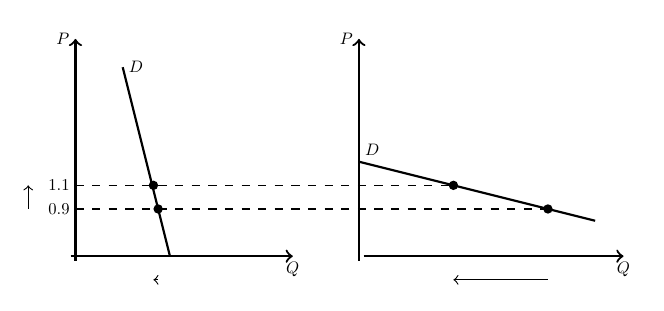
\begin{tikzpicture}[
			scale = 0.6,
			every node/.style={scale = 0.6}]

			\draw[->,thick] (-0.1,0) -- (4.6,0)node[below]{$Q$};
			\draw[->,thick] (0,-0.1) -- (0,4.6)node[left]{$P$};

			\draw[->,thick] (6.1,0) -- (11.6,0)node[below]{$Q$};
			\draw[->,thick] (6,-0.1) -- (6,4.6)node[left]{$P$};

			\draw[thick](1,4)node[right]{$D$}--(2,0);
			\draw[thick](6,2)node[above right]{$D$} -- (11,0.75);

			\draw[dashed](0,1.5)node[left]{$1.1$} -- (1.65,1.5) node[circle,fill,inner sep= 2pt]{} -- (8,1.5)node[circle,fill,inner sep=2pt]{};
			\draw[dashed](0,1)node[left]{$0.9$} -- (1.75,1) node[circle,fill,inner sep= 2pt]{} -- (10,1)node[circle,fill,inner sep=2pt]{};

			\onslide<2->{
				\draw[->](-1,1) -- (-1,1.5);
				\draw[->](1.75,-0.5) -- (1.65,-0.5);
				\draw[->](10,-0.5) -- (8,-0.5);
			}

		\end{tikzpicture}  
	\end{center}

\end{frame}

\begin{frame}
	\frametitle{Casos interm\'edios}
	Se no primeiro caso, $Q$ passa de 85 para 80, e no segundo caso $Q$ pasa de 205 para 95 obtemos o seguinte:
	\begin{align*}
		|\varepsilon_D|=\left|\frac{80-85}{1.1-0.9}\frac{\frac{1.1+0.9}{2}}{\frac{80+85}{2}}\right|=0.3
	\end{align*}

	Ou seja procura inel\'astica!

	Assim, para o segundo caso teremos:
	\begin{align*}
		|\varepsilon_D|=\left|\frac{95-205}{1.1-0.9}\frac{\frac{1.1+0.9}{2}}{\frac{205+95}{2}}\right|=3.7
	\end{align*}

	Ou seja procura el\'astica!
\end{frame}